\documentclass{report}

\usepackage[T1]{fontenc} % Fontes T1
\usepackage[utf8]{inputenc} % Input UTF8
\usepackage[backend=biber, style=ieee]{biblatex} % para usar bibliografia
\usepackage{SIunits}
\usepackage{csquotes}
\usepackage[portuguese]{babel} %Usar língua portuguesa
\usepackage{blindtext} % Gerar texto automaticamente
\usepackage[printonlyused]{acronym}
\usepackage{hyperref} % para autoref
\usepackage{graphicx}
\usepackage{float}
\usepackage{biblatex} 

\bibliography{bibliografia}


\begin{document}
%%
% Definições
%%
\def\titulo{Incêndios}
\def\data{\today}
\def\autores{Renato Valente, Ruben Menino}
\def\autorescontactos{(89077) renatovalente5@ua.pt, (89185) ruben.menino@ua.pt}
\def\versao{V1.0}
\def\departamento{DEPARTAMENTO}
\def\empresa{DETI - Universidade de Aveiro}
\def\logotipo{ua.pdf}
%
%%%%%% CAPA %%%%%%
%
\begin{titlepage}

\begin{center}
%
\vspace*{50mm}
%
{\Huge \titulo}\\ 
%
\vspace{10mm}
%
{\Large \empresa}\\
%
\vspace{10mm}
%
{\LARGE \autores}\\ 
%
\vspace{30mm}
%
\begin{figure}[h]
\center
\includegraphics{\logotipo}
\end{figure}
%
\vspace{30mm}
\end{center}
%
\begin{flushright}
\versao
\end{flushright}
\end{titlepage}

%%  Página de Título %%
\title{%
{\Huge\textbf{\titulo}}\\
{\Large \departamento\\ \empresa}
}
%
\author{%
    \autores \\
    \autorescontactos
}
%
\date{\data}
%
\maketitle

\pagenumbering{roman}

%%%%%% RESUMO %%%%%%
\begin{abstract}
Cada vez mais os incêndios têm atingido Portugal, tornando-se no país com um número maior de incêndios na Europa. Como consequência dos incêndios vêm a destruição de hectares de terrenos, pondo em risco as habitações das pessoas e as suas vidas. Recentemente ocorreu um dos maiores incêndios na história de Portugal em Pedrógão Grande, provocando 64 mortes e a destruição de uma vasta área, cerca de 30.000 hectares. O surgimento de fumos e do aumento de calor devido aos incêndios podem trazer problemas a nível da saúde das populações que se encontram nessas zonas. Existem medidas para tentar diminuir não só o número de incêndios, como também a dimensão dos hectares ardidos. Não fazer queimadas, lançamento de foguetes, fogueiras… são algumas das formas para prevenir a incidência de incêndios. As populações afetadas pelos incêndios, em que devido ao fogo perderam as suas casas e os seus bens, são previligiadas com apois do Ministério da Justiça e do Ministério da Saúde, de forma a poderem reestruturar as suas vidas, sendo-lhes fornecido apoio material, psicologico e alimentar, de forma a satisfazer as nessecidades basicas. 
\end{abstract}

%%%%%% Agradecimentos %%%%%%
\renewcommand{\abstractname}{Agradecimentos}
\begin{abstract}
Gostaríamos de agradecer, em primeiro lugar, ao professor João Paulo Silva Barraca pela lecionação da matéria e das dúvidas que nos esclareceu para a realização deste trabalho. Gostaríamos de agradecer aos nossos colegas pela disposição e partilha de informações e também às fontes usadas que nos permitiram concluir a realização deste trabalho.
\end{abstract}


\tableofcontents
% \listoftables     % descomentar se necessário
% \listoffigures    % descomentar se necessário


%%%%%%%%%%%%%%%%%%%%%%%%%%%%%%%
\clearpage
\pagenumbering{arabic}

%%%%%%%%%%%%%%%%%%%%%%%%%%%%%%%%%%%%%%%%%%%%%%%%%%%%%%%%%%%%%%%%

\chapter{Introdução}

Este trabalho foi realizado no âmbito da unidade curricular Laboratórios de Informática, esta que é lecionado pelo Professor Paulo Barraca. Foi solicitado à turma a elaboração de grupos para posteriormente se proceder à realização de um trabalho. O tema escolhido pelo nosso grupo foi “Incêndios”.
Na elaboração deste trabalho pretende-se que seja recolhido o máximo de informação credível e pertinente.
Sendo assim, podemos definir como principais objetivos: adquirir conhecimentos relativamente ao tema em questão; elaborar estratégias de modo a processar a informação para que seja facilmente percetível e compreensível ao leitor; Analisar os \autoref{dados estatísticos relacionados nos incêndios}; Dar a cohecer medidas para a \autoref{prevenção de incêndios}; Ter conhecimentos dos \autoref{riscos para a saúde associados ao fumo produzido pelos incêndios}, dos \autoref{problemas relacionados com o excesso de calor}, dos \autoref{problemas relacionados com as falhas no abastecimento de água}, \autoref{apoios à população após incêndios e prevenção de incêndios}, \autoref{tipos de queimaduras} que os incêndios poderão provocar .
A informação foi inserida neste documento de uma forma sequencial e lógica para que exista uma boa organização dos conteúdos, facilitando a compreensão dos mesmos.

%%%%%%%%%%%%%%%%%%%%%%%%%%%%%%%%%%%%%%%%%%%%%%%%%%%%%%%%%%%%%%%%%

\chapter{Dados estatísticos relacionados nos incêndios}
\label{dados estatísticos relacionados nos incêndios};
\cite{ICNF}

Existem diversas entidades responsáveis pelo estudo estatístico dos incêndios, como o Instituto Nacional de Estatística, Proteção Civil Portugal, Instituto de conservação da natureza e das florestas e \ac{gnr}
Estes dados obtidos permitem a análise a diversos aspetos como as causas dos incêndios, o número de incêndios florestais e a quantidade de área ardida num determinado ano.

\begin{figure}[H]
\center
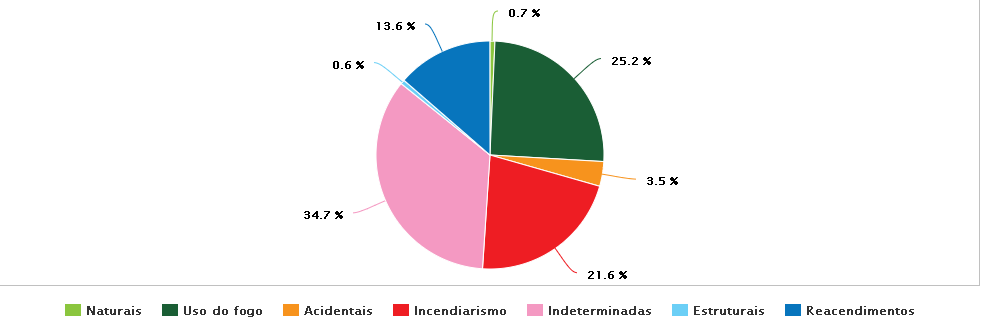
\includegraphics[width=10cm]{circular.png}
\caption{Causas dos incêndios florestais investigados pela \ac{gnr}}
\end{figure}

Segundo os dados obtidos podemos verificar que apenas uma ínfima percentagem de incêndios florestais é de causa natural.
Verifica-se também que cerca de 22\% dos incêndios têm obra de mão criminosa.
Relativamente as causas acidentais e por uso do fogo verificamos que tem uma grande percentagem associada (28,7\%), estes são causados muitas vezes por negligência. É essencial que se atue ao nível da prevenção para diminuir esta percentagem, para isso é importante a divulgação de informação de modo a alertar as populações dos cuidados que devem ser tomados para a prevenção de possíveis incêndios (\ac{icnf},2016).

\begin{figure}[H]
\center
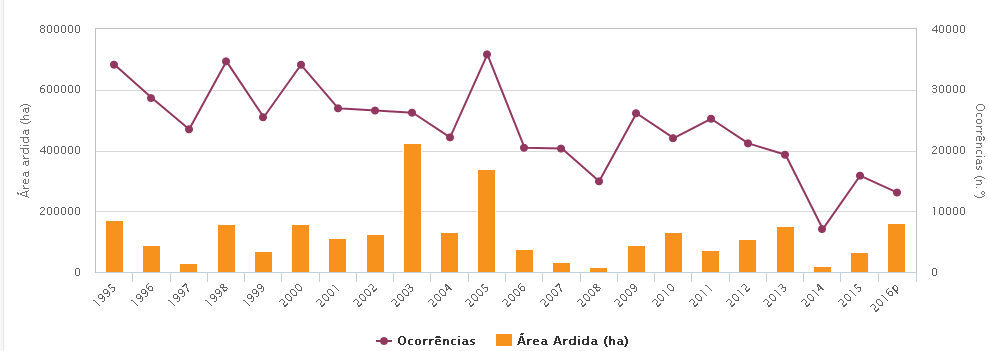
\includegraphics[width=10cm]{barras.png}
\caption{Número de incêndios florestais e área ardida em hectares.}
\end{figure}

Analisando o gráfico apresentado podemos verificar que os números de incêndios florestais têm diminuindo significativamente desde 1995 até ao ano de 2016. Estes números apresentados devem-se á maior divulgação de informação á população relativa á prevenção dos incêndios, como a proibição de queimadas em determinadas alturas do ano e todos os cuidados que a população deve tomar de modo a evitar estas ocorrências (\ac{icnf},2016).

%%%%%%%%%%%%%%%%%%%%%%%%%%%%%%%%%%%%%%%%%%%%%%%%%%%%%%%%%%%%%%%%%

\chapter{Prevenção de Incêndios}
\label{prevenção de incêndios}
\cite{dgsefeitos-fumo}

A cada ano que decorre o número de incêndios em Portugal é cada vez mais frequente, é importante desta forma apostar recursos na prevenção dos mesmos. A intervenção do homem na prevenção é essencial de modo a evitar a origem dos incêndios bem como evitar o desenvolvimento dos mesmos. Segundo a Proteção Civil existem algumas situações em que é necessária uma maior prevenção por parte da população, de modo a diminuir a incidência dos incêndios:
\begin{enumerate}
 \item Queimadas
 \item Lançamento de foguetes
 \item Utilização de fósforos e cigarros
 \item Fogueiras
 \item Piqueniques
 \item Apicultura
 \item Linhas elétricas
 \item Vias férreas
 \item Rede viária
 \item Máquinas ou equipamento de motor ou combustão
 \item Chaminés
\end{enumerate}

A Proteção Civil salienta a importância dos cuidados a ter na realização das queimadas, tendo em conta diversos aspetos que devem ser respeitados como, temperatura do ar ambiente, humidade, vento, vigilância e água de modo a prevenir casos de emergência, na realização de queimadas.

%%%%%%%%%%%%%%%%%%%%%%%%%%%%%%%%%%%%%%%%%%%%%%%%%%%%%%%%%%%%%%%%%

\chapter{Riscos para a saúde resultantes da ocorrência de incêndios}
\cite{dgsefeitos-fumo}

Os incêndios florestais são considerados catástrofes ambientais. Estas catástrofes são responsáveis por prejuízos económicos e ambientais acrescidos, mas acima de tudo constituem um risco para todas as populações e para a saúde das mesmas.



\section{Riscos para a saúde associados ao fumo produzido pelos incêndios}
\label{riscos para a saúde associados ao fumo produzido pelos incêndios}
\cite{dgsefeitos-fumo}

Ao analisar os componentes tóxicos presentes no fumo verificamos que estes dependem na sua grande maioria dos materiais envolvidos e se estes ardem completamente, ou se apenas são derretidos. Também a presença de vento e a sua direção pode ajudar ou não a combustão completa e também a disseminação das partículas a grande distância.
 Averiguando a constituição do fumo libertado nos incêndios, observamos que este é constituído por vapor de água, por monóxido de carbono (\ac{co}), óxido nítrico (\ac{no3}), dióxido de carbono (\ac{co2}), compostos orgânicos voláteis irritantes (COV) (tóxicos do ar e partículas muito pequenas: PM2,5 e PM10).
Relativamente aos gases verificamos que, quanto ao monóxido de carbono (\ac{co}), tem a capacidade de penetrar rapidamente na corrente sanguínea através dos pulmões e de se combinar irreversivelmente com a hemoglobina, substância responsável pelo transporte do oxigénio para os tecidos humanos. Para aqueles que sofrem de doenças cardiovasculares o perigo é muito mais sério, pois em níveis elevados de \ac{co}, poderá levar a dores de cabeça, tonturas, perturbações da visão, redução da capacidade de trabalho e diminuição da destreza manual.
O dióxido de enxofre (\ac{so2}) é um gás irritante para as mucosas dos olhos, nariz e garganta. A exposição em demasia a este poluente pode afetar o sistema respiratório, provocando alterações nos mecanismos de defesa dos pulmões e agravar doenças como a asma, bronquite crónica e doenças cardiovasculares já existentes. Por outro lado, o dióxido de enxofre poderá ser transformado em gotículas de acido sulfúrico o que lavará a uma maior irritação na mucosa respiratória.
O dióxido de nitrogénio (\ac{no2}) é libertado durante a combustão a temperaturas elevadas e poderá desencadear um aumento da reatividade brônquica que se traduz muitas vezes em crise de falta de ar em indivíduos com asma.

\begin{figure}[H]
\center
\includegraphics[width=10cm]{fumo.jpg}
\caption{Exposição ao fumo dos incêndios florestais.}
\end{figure}


O ozono (\ac{o3}) poderá causar irritação do nariz, da garganta e da traqueia. E por fim o ácido cianídrico poderá provocar sintomas como confusão mental, taquicardia e respiração acelerada. 
Por outro, a principal ameaça para a saúde resultante do fumo provém das partículas. As partículas com um diâmetro inferior a 10\micro\meter (PM 10), poderão conduzir a situações como tosse, irritação nos olhos, nariz e garganta, até mesmo ao aparecimento de doenças pulmonares crónicas obstrutivas. Além disso, são as partículas com diâmetro inferior a 2.5 \micro\meter (PM 2,5) que provocam problemas mais graves, uma vez que estas são pequenas o suficiente para serem inaladas e entrarem mais profundamente nos pulmões, provocando assim doenças respiratórias como asma, ou até mesmo penetrar na corrente sanguínea provocando a morte (\ac{dgs},2011).
Segundo a \ac{dgs} é importante informar a população relativamente aos riscos associados á exposição de fumos e assim lançar medidas de prevenção. Como resposta, a direção geral de saúde lançou um comunicado no dia 17/08/2017 que foca em alguns pontos essenciais. Desta forma, a \ac{dgs} recomenda á população que evite a exposição ao fumo, evitando atividades a ar livre, salienta a importância da utilização de máscaras, sempre que for inevitável a exposição ao fumo, toma continua da medicação habitual para doentes com problemas a nível respiratório e manter-se hidratado e informado [ CITATION Fra17 \l 2070 ].


\section{Problemas relacionados com o excesso de calor}
\label{problemas relacionados com o excesso de calor}
\cite{dgsriscos}

Como sabemos, verifica-se um maior número de incêndios durante os meses do verão, estes que são também característicos pelo facto de levarem à existência de um aumento da temperatura. Este aumento da temperatura que se verifica no verão em conjunto com o calor provocado pela ocorrência de incêndios leva à existência de problemas de saúde pública associados a essa situação.

\begin{figure}[H]
\center
\includegraphics[width=10cm]{calor.jpg}
\caption{Alerta devido ao calor e riscos de incêndios.}
\end{figure}



Apesar de todos os indivíduos possam ser afetados com o excesso de calor que se pode fazer sentir devido à ocorrência de incêndios, existem alguns grupos populacionais que estão mais sujeitos aos efeitos provocados por esse excesso de calor, são estes: "As crianças nos primeiros anos de vida, as pessoas idosas e os portadores de doenças crónicas, nomeadamente os que sofrem de afeções cardíacas, respiratórias, renais, diabetes, obesidade e doença mental" (\ac{dgs},2011).
O excessivo calor que se pode fazer sentir quando estamos perante situações de incêndios, poderão levar há ocorrência de problemas considerados como "Emergências Médicas". Sendo assim, as emergências médicas que poderão ser desencadeadas devido ao calor excessivo são:

\begin{itemize}
\item (Cãimbras) Caso a pessoa, que tenha estado sujeita a elevadas temperaturas, comece a ter cãibras, deverá: afastar-se da causa que está a provocar o aumento da temperatura, e de seguida procurar um sitio mais fresco, arejado e calmo. Deve também promover uma boa hidratação.

\begin{figure}[H]
\center
\includegraphics[width=10cm]{caimbras.jpg}
\caption{Cãimbras nas pernas}
\end{figure}

Se as cãibras não passarem ao fim de uma hora, deverá dirigir-se a uma unidade de cuidados de saúde (\ac{dgs},2011).

\item (Golpe de calor) O golpe de calor é considerado uma emergência médica, pelo facto de se caraterizar pela incapacidade de o corpo humano não conseguir controlar a sua própria temperatura, levando a elevações de temperatura de tal forma extremas que podem desencadear deficiências crónicas ou mesmo a morte. O corpo não consegue regular a temperatura corporal pelo facto de ser perdida a capacidade de sudação. As temperaturas poderão atingir mesmo os 39ºC em 10 a 15 minutos.
Em caso de presença dos sintomas anteriormente referidos deverá: “Procurar ajuda numa unidade de cuidados de saúde, com o objetivo de arranjar mecanismos para diminuir a temperatura corporal; Procurar um local mais fresco e usar meios para arrefecimento natural, tais como banho de agua fria ou tépida; Se ocorrerem contrações corporais, não devem ser administrados líquidos e deverá prevenir-se que a pessoa se magoe;” (\ac{dgs},2011).

\item (Esgotamento devido ao calor) O esgotamento provocado pelo excesso de calor, deve-se ao facto de haver uma excessiva perda de líquidos e sódio pela sudação, e é um problema que poderá ser mesmo fatal em idosos e pessoas que sofram de hipertensão arterial.

\begin{figure}[H]
\center
\includegraphics[width=10cm]{esgotamentocalor.jpg}
\caption{Esgotamento devido ao calor}
\end{figure}



Caso se verifique a ocorrência destes sintomas, a pessoa deverá: “Procurar ajuda numa unidade de cuidados de saúde o mais rapidamente possível. Caso a pessoa sofra de problemas cardíacos ou hipertensão é necessário que a procura de ajuda médica imediata; Enquanto se espera pela prestação de cuidados de saúde, deverá ser feito arrefecimento, promover a hidratação da pessoa e o seu repouso;” (\ac{dgs},2011).
\end{itemize}

\section{Problemas relacionados com as falhas no abastecimento de água}
\label{problemas relacionados com as falhas no abastecimento de água}
\cite{dgsriscos}

A água é um bem essencial e imprescindível na nossa vida, seja para consumo próprio ou para evitar a devastação da nossa floresta. Com a chegada dos incêndios chegam também os problemas no abastecimento de água. 
Por vezes, ocorrem alterações na qualidade da água devido aos incêndios e ao efeito que eles provocam no meio ambiente. Dessa forma, é necessário recorrer a outros meios de abastecimento, os chamados meios alternativos, com o objetivo de não colocar em risco a saúde das pessoas que estão envolvidos neste fenómeno ambiental. A passagem facilitada da água para o subsolo devido à perda de vegetação, consequente dos incêndios, levará a um conjunto de transformações químicas, como a entrada de sedimentos e cinzas nos fluxos de água, que a irão tornar imprópria para o consumo da população e constituir um grande risco para a saúde pública.
De forma preventiva, é necessário elaborar um conjunto de medidas alternativas às habituais, com o objetivo de contornar/reduzir os riscos para a saúde humana  (\ac{dgs},2011).


\subsection{Protocolos de desinfeção da água - Medidas a incrementar}

\subsubsection{Fervura de água destinada a consumo humano}
\cite{dgsriscos}

Grande parte dos microrganismos patogénicos e prejudiciais para a saúde do Homem não conseguem sobreviver e proliferar em ambientes com altas temperaturas. Assim, a fervura da água contaminada é um método executado muito frequentemente e que é bastante eficiente na eliminação de bactérias, fungos, parasitas, entre outras. De seguida a água deverá ser armazenada num recipiente fechado e colocada num ambiente fresco(\ac{dgs},2011).(Figura\ref{agua})

\begin{figure}[H]
\center
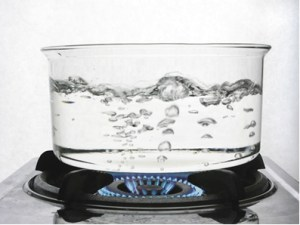
\includegraphics[width=3cm]{agua.jpg}
\caption{Água a ferver.(\cite{figagua})}
\label{agua}
\end{figure}

\subsubsection{Desinfeção Química}
\cite{dgsriscos}

A desinfeção da água é executada através de produtos à base de cloro e iodo. Normalmente, é utilizada uma lixivia comercial à escolha do consumidor para uma desinfeção adequada, desde que não contenha corantes, nem qualquer tipo de detergentes. (Tabela\ref{tab1}  Figura\ref{quimi})

\begin{table}
\centering
\caption{Uso doméstico de lixivias comerciais de acordo com a concentração de hipoclorito sódio e da quantidade de água.(}
\begin{tabular}{|c||c||c|}
\hline
\textbf{Concentraçao lixívia(\%)}     &  \textbf{1 litro}  &  \textbf{2 litros}  \\ \hline
	\textbf{1\%}		      &  4 gotas	   &  8 gotas   \\ \hline
	\textbf{2\%}		      &	 2 gotas	   &  4 gotas   \\ \hline
	\textbf{4\%}		      &  1 gota	       &  2 gotas   \\ \hline
	\textbf{8\%}		      &     -    	   &  1 gota    \\ \hline
	\textbf{10\%}		      &     -    	   &  1 gota    \\ \hline
\end{tabular}
\label{tab1}
\end{table}



\begin{figure}[H]
\center
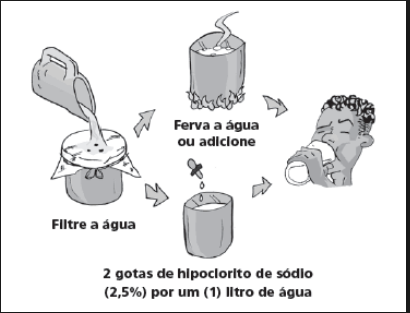
\includegraphics[width=7cm]{pic2.png}
\caption{Água a ferver.(\cite{fquim})}
\label{quimi}
\end{figure}


%%%%%%%%%%%%%%%%%%%%%%%%%%%%%%%%%%%%%%%%%%%%%%%%%%%%%%%%%%%%%%%%%

\chapter{Apoios a população após incêndios}
\label{apoios à população após incêndios e prevenção de incêndios}
\cite{pgov2017}

\begin{enumerate}
 \item Ministério da Justiça:\\
 O Ministério da Justiça em conjunto com o Ministério de Planeamento e Infraestruturas e com o Ministério das Finanças desenvolveu um programa que consiste em dispensar procedimentos e taxas e possibilita o cancelamento oficioso de matrículas e registos de veículos danificados pelos incêndios, sem necessidade de um pedido dos interessados e quaisquer deslocações às Conservatórias ou ao Instituto da Mobilidade e dos Transportes.
 
\begin{figure}[H]
\center
\includegraphics[width=3cm]{justiça.jpg}
\caption{Ministério da Justiça}
\label{agua}
\end{figure} 
 
  Ainda com o envolvimento da Autoridade Tributária, vem assim evitar que os titulares falecidos ou os familiares recebam notificações para liquidação do Imposto Único de Circulação.
 
 \item Segurança Social :\\
 Atribuição de “subsídios de caráter eventual, de concessão única ou de manutenção, de apoio aos indivíduos e às famílias que se encontrem em situação de carência ou perda de rendimento e que necessitem de proceder a despesas necessárias à sua subsistência ou à aquisição de bens imediatos e inadiáveis”[ CITATION Rep17 \l 2070 ], nomeadamente:
 \begin{itemize}
 
  \item Despesas com rendas em situações de alojamento para habitação temporária; 
  \item Aquisição de bens e serviços de primeira necessidade nas áreas de alimentação, vestuário, habitação, saúde, educação e transportes; 
  \item Aquisição de instrumentos de trabalho; 
  \item Aquisição de ajudas técnicas/produtos de apoio; 
  \item Aquisição de outros bens e serviços ou realização de despesas considerados necessários após avaliação pelos serviços competentes da segurança social.
  
 \end{itemize}
 
 \item Ministério da saúde
 \begin{itemize}
  \item Fornecimento de apoio psicológico por equipas de Saúde Mental Comunitária (psiquiatras, psicólogos clínicos, enfermeiros e técnicos de Serviço Social); 
  \item Avaliação dos efeitos na saúde da população exposta aos incêndios por Equipas de Saúde Pública, que contam com médicos de saúde pública e técnicos de saúde Ambiental;
  \item Nos Cuidados de Saúde Primários, os recursos humanos são ajustados à procura, quer de consultas de agudos quer de consultas programadas.
  
 \end{itemize}
 
 \item Criação Linha Nacional de Emergência Social (\ac{lnes})\\
  Esta linha, acessível através do número 144, foi desenvolvida em articulação entre os Ministérios da Justiça, Trabalho Solidariedade e Segurança Social e Saúde. Tendo por base que o “Cidadão deve encontrar um ponto de contacto e resposta imediata à sua exposição com o agendamento de uma data/hora para se deslocar a um serviço da sua conveniência, onde o aguardam técnicos habilitados para a resolução do problema específico identificado na triagem telefónica” (Republica Portuguesa, 2017).
  
\begin{figure}[H]
\center
\includegraphics[width=3cm]{144.jpg}
\caption{Linha Nacional de Emergência Social - LNES - 144}
\label{agua}
\end{figure}  
  
Permitindo assim, às populações poderem obter acompanhamento social, subsídios eventuais, encaminhamento para resposta social, prestações sociais ou apoios sociais específicos, apoio psicológico e encaminhamento para cuidados de saúde (Republica Portuguesa, 2017).


 \end{enumerate}

 %%%%%%%%%%%%%%%%%%%%%%%%%%%%%%%%%%%%%%%%%%%%%%%%%%%%%%%%%%%%%%%%%
 
\chapter{Tipos de Queimaduras} 
\label{tipos de queimaduras}
\cite{dgsriscos}

Durate os incêndios, as pessoas que os cambatem, quer seja bombeiro ou civil,  estam sujeitas ao contacto da chama com a pele, podendo provocar queimaduras de diferentes graus.
As queimaduras classificam-se de acordo com a sua profundidade e o tamanho destas.
Na tabela a seguir podemos observar os diferentes graus de queimaduras. (Tabela\ref{tab2}  Figura\ref{queimaduras})

\begin{figure}[H]
\center
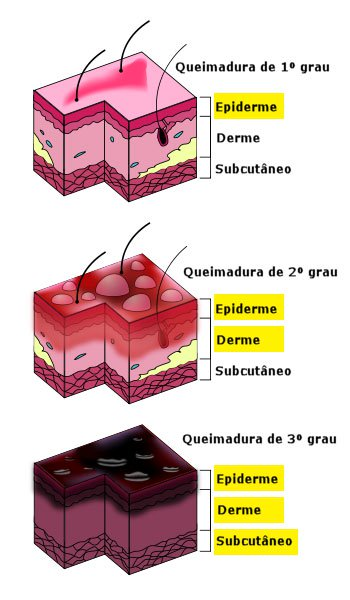
\includegraphics[width=3cm]{queimaduras.jpg}
\caption{Tipos de Queimaduras.(\cite{fquei})}
\label{queimaduras}
\end{figure}



\begin{table}
\caption{Características das queimaduras}
\centering
\begin{tabular}{|c||c||c|}
\hline  
   \textbf{1ºGrau}	  	&  \textbf{2ºGrau}	  &  \textbf{3ªGrau}		 \\  \hline
   Atinge a epiderme		&  Atinge a derme         &  Destruição dos tecidos \\  \hline
   Causa Vermelhidão da pele   	&  Ardor intenso	  &  Nesseçário apoio médico \\  \hline
   Não há formação de bolhas    &  Há formação de bolhas  &  A pele fica carbonizada \\  \hline
\end{tabular}
\label{tab2}
\end{table}
 %%%%%%%%%%%%%%%%%%%%%%%%%%%%%%%%%%%%%%%%%%%%%%%%%%%%%%%%%%%%%%%%%
 
\chapter{Reflexão crítica}
Sendo Portugal o país europeu com mais área ardida na última década, verificou-se este ano a época mais crítica de incêndios florestais no nosso país, sendo que mais de 230 mil hectares de área arderam.
Durante esta época de incêndios abordou-se bastante as falhas no funcionamento do Sistema Integrado de Redes de Emergência e Segurança de Portugal, que começaram no incêndio de Pedrógão Grande e repetiram-se, pelo menos, nos fogos de Alijó, Abrantes, Mealhada, Cantanhede e no distrito de Castelo Branco.
O nosso grupo tem por opinião, que para que seja alterado a tendência de aumento das áreas ardidas serão necessárias medidas a longo-prazo, onde estas só irão ter sucesso se forem assumidas por todos, enquanto objetivo estratégico do desenvolvimento global do país.
Para além das boas medidas de política, existe também a necessidade de envolvimento dos cidadãos, mais particularmente, das populações, seguindo-se de um esforço de esclarecimento e mobilização.
Consideramos ainda, que é imprescindível a adoção de um Plano Nacional de Defesa da Floresta Contra Incêndios.
Por fim, tendo em conta a quantidade de pessoas lesadas tanto direta como indiretamente devido aos incêndios, a quantidade de mortes que ocorreram, de bens que foram perdidos devido às chamas, gostaríamos então de apelar a uma planificação de estratégias com vista a diminuir a quantidade de incêndios que ocorrem. 




%%%%%%%%%%%%%%%%%%%%%%%%%%%%%%%%%%%%%%%%%%%%%%%%%%%%%%%%%%%%%%%%%

\chapter{Conclusão}
Hoje em dia cada vez podemos observar com maior frequência a ocorrência de incêndios, onde uma considerável percentagem seja por responsabilidade das pessoas. Verificando assim que o Ser Humano acaba por se prejudicar a si próprio e aos seus chegados. Isto contando com todos os efeitos precedentes dos incêndios, tanto físicos para quem os combate e por quem é “rodeado” por estes, como também psicológicos para quem perde um próximo, para quem perde pertences como as suas casas ou até mesmo só pelas imagens que são capturadas tanto ao vivo como pela comunicação social.
Posto isto, é importante salientar e consequentemente alertar a população afetada sobre os riscos para a saúde derivados destas catástrofes. Prevenindo assim, a ocorrência de complicações com a diminuição da recorrência a unidades de saúde. Não pondo de parte a importância da ajuda necessária às populações que acabam por ser envolvidas e prejudicadas por este fenómeno.
Em suma, os objetivos definidos neste trabalho foram alcançados com sucesso, podendo o grupo reter informação deste fenómeno ambiental e consciencializando-se um pouco mais da realidade que são os incêndios, os seus riscos e as suas consequências devastadoras.



%%%%%%%%%%%%%%%%%%%%%%%%%%%%%%%%%%%%%%%%%%%%%%%%%%%%%%%%%%%%%%%

\chapter*{Acrónimos}

\begin{acronym}
 \acro{dgs}[DGS]{Direção-Geral da Saúde}
 \acro{gnr}[G.N.R]{Guarda Nacional Republicana}
 \acro{icnf}[ICNF]{Instituto de Conservação da Natureza e das Florestas}
 \acro{co}[CO]{monóxido de carbono}
 \acro{no3}[NO3]{óxido nítrico}
 \acro{co2}[CO2]{dióxido de carbono}
 \acro{cov}[COV]{compostos orgânicos voláteis}
 \acro{so2}[SO2]{dióxido de enxofre}
 \acro{no2}[NO2]{dióxido de nitrogénio}
 \acro{o3}[O3]{ozono DGS- Direção Geral de Saúde}
 \acro{lnes}[LNES]{Linha Nacional de Emergência Social}
\end{acronym}
 
%%%%%%%%%%%%%%%%%%%%%%%%%%%%%%%%%%%%%%%%%%%%%%%%%%%%%%%%%%%%%%%%%


\printbibliography

\end{document}